\section{Key exchange protocol}\label{sec:keyxchng}

\figref{fig:keyxchng} shows the sequence diagram of a session with three
parties: Alice (client), Bob (client) and the Server.

\begin{figure}[htb]
	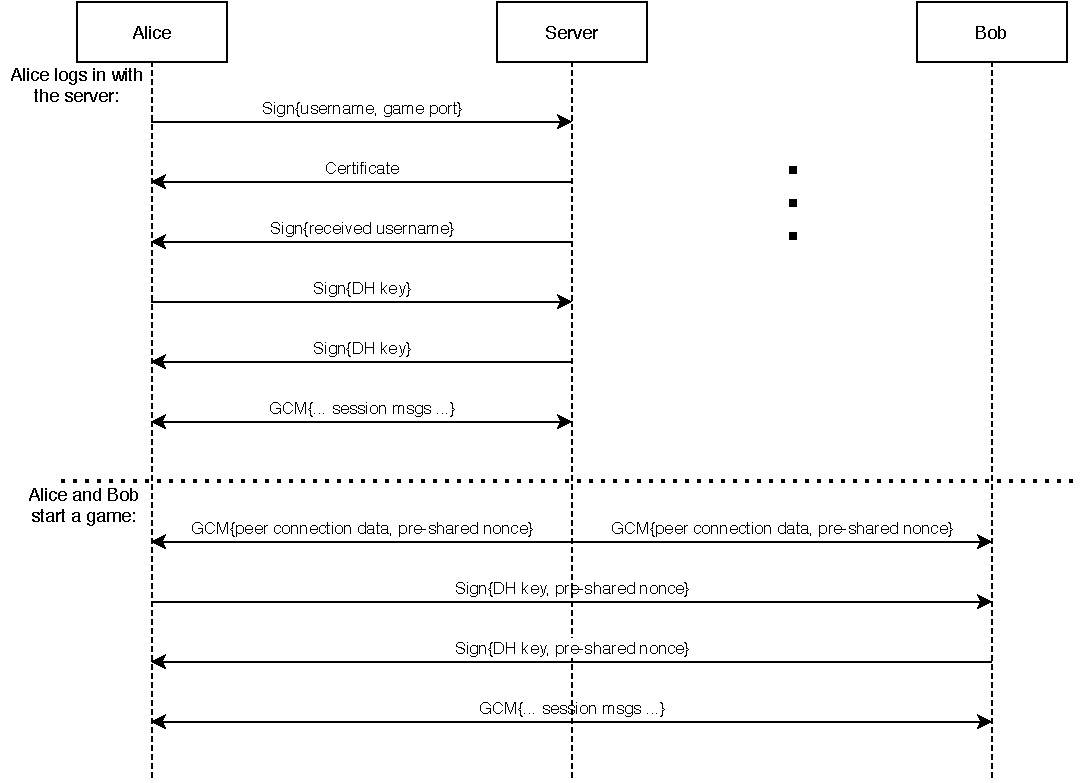
\includegraphics[width=\textwidth]{keyxchng}
	\caption{Sequence diagram of a sample session}\label{fig:keyxchng}
\end{figure}

In the figure only the content of the body part of messages are represented: the
header for each message is always the one shown in \lstref{lst:msgheader}.

\subsection{Formal description}\label{subsec:formal}

In the following we will simplify the protocol messages to only contains the
informations needed to guarantee the security of the protocol (in the real
protocol, each field of the header is always included even when it is not
useful).

\subsubsection{Notation}

\begin{itemize}
	\item \(A\) is a client, also named ``Alice'';
	\item \(B\) is another client, also named ``Bob'';
	\item \(S\) is the server;
	\item \(\mathit{CA}\) is the certification authority;
	\item \(N_P^n\) is a random nonce generated by the principal \(P\). The
		superscript \(n\) is used to distinguish between different
		nonces;
	\item \(\hash(X)\) means ``the hash of \(X\)'';
	\item \(\hash(\ldots)\) means ``the hash of the current message''. So,
		when we write \(\sign{\hash(\ldots)}{K}\) we mean that the
		message is hashed and then the hash is signed with \(K^{-1}\).
		This represents the work done by the EVP API of \openssl;
	\item \(\mathit{DHKEY}_P^{PQ}\) is the Diffie-Hellman public key
		generated by the principal \(P\) for use in the communication
		between \(P\) and \(Q\);
	\item \(\mathit{DH}_{params}\) are the Diffie-Hellman pre-shared
		parameters (\(p\) and \(g\));
	\item \(K_{GCM}^{PQ}\) is the shared GCM key between \(P\) and \(Q\)
		derived from the shared secret obtained from Diffie-Hellman.
\end{itemize}

\subsubsection{Idealized protocol}

Here we assume that there are no errors and the client successfully
authenticates with the server:
\begin{itemize}
	\item[M1:] \(A \sends S \qquad \sign{N_A^1, A, port}{K_A}\)
	\item[M2:] \(S \sends A \qquad N_S^1, \sign{K_S^{-1}}{K_{CA}}, \hash(M1)\)
	\item[M3:] \(S \sends A \qquad N_S^2, A, \hash(M1), \sign{\hash(\ldots)}{K_S}\)
	\item[M4:] \(A \sends S \qquad N_A^2, \mathit{DHKEY}_A^{AS}, \hash(M3), \sign{\hash(\ldots)}{K_A}\)
	\item[M5:] \(S \sends A \qquad N_S^3, \mathit{DHKEY}_S^{AS}, \hash(M4), \sign{\hash(\ldots)}{K_S}\)
\end{itemize}

At this point the session key for GCM is derived (\(K_{GCM}^{AS}\)). Here we will
show the continuation of the protocol when Alice asks to challenge Bob. For
simplicity, we do not show the message that the server sends to Bob with the
challenge request and the response for accepting/refusing it (like if the
challenge is automatically accepted by Bob):
\begin{itemize}
	\item[M6:] \(A \sends S \qquad \encrypt{N_A^3, \mathit{CHALL\_REQ}, B, \hash(M5)}{K_{GCM}^{AS}}\)
	\item[M7:] \(S \sends A \qquad \encrypt{N_S^4, \mathit{address}_B, K_B^{-1}, N_{DH}, \hash(M6)}{K_{GCM}^{AS}}\)
	\item[M8:] \(S \sends B \qquad \encrypt{N_S^5, \mathit{address}_A, K_A^{-1}, N_{DH}, \hash(\mathit{prev\,msg\,from\,B})}{K_{GCM}^{BS}}\)
	\item[M9:] \(A \sends B \qquad N_A^4, \mathit{DHKEY}_A^{AB}, \sign{\hash(\ldots)}{K_A}\)
	\item[M10:] \(B \sends A \qquad N_B^1, \mathit{DHKEY}_B^{AB}, \hash(M9), \sign{\hash(\ldots)}{K_B}\)
	\item[M11:] \(A \sends B \qquad \encrypt{N_A^5, \mathit{GAME\_MOVE}_A, \hash(M10)}{K_{GCM}^{AB}}\)
	\item[M12:] \(B \sends A \qquad \encrypt{N_B^2, \mathit{GAME\_MOVE}_B, \hash(M11)}{K_{GCM}^{AB}}\)
\end{itemize}

\subsubsection{Assumptions}

\begin{itemize}
	\item \(A \believes \fresh{N_A^n}\) for each \(n \in \mathbb{N}\)
	\item \(B \believes \fresh{N_B^n}\) for each \(n \in \mathbb{N}\)
	\item \(S \believes \fresh{N_S^n}\) for each \(n \in \mathbb{N}\)
	\item \(A \believes S \controls N_S^n\) for each \(n \in \mathbb{N}\)
	\item \(B \believes S \controls N_S^n\) for each \(n \in \mathbb{N}\)
	\item \(S \believes A \controls N_A^n\) for each \(n \in \mathbb{N}\)
	\item \(S \believes B \controls N_B^n\) for each \(n \in \mathbb{N}\)
	\item \(A \believes B \controls N_B^n\) for each \(n \in \mathbb{N}\)
	\item \(B \believes A \controls N_A^n\) for each \(n \in \mathbb{N}\)
	\item \(S \believes \pubkey{K_A} A\)
	\item \(S \believes \pubkey{K_B} B\)
	\item \(A \believes \pubkey{K_{CA}} \mathit{CA}\)
	\item \(B \believes \pubkey{K_{CA}} \mathit{CA}\)
	\item \(A \believes \mathit{CA} \controls \pubkey{K_S} S\)
	\item \(B \believes \mathit{CA} \controls \pubkey{K_S} S\)
	\item \(A \believes A \secret{\mathit{DH}_{params}} S\)
	\item \(S \believes S \secret{\mathit{DH}_{params}} A\)
	\item \(B \believes B \secret{\mathit{DH}_{params}} S\)
	\item \(S \believes S \secret{\mathit{DH}_{params}} B\)
	\item \(A \believes A \secret{\mathit{DH}_{params}} B\)
	\item \(B \believes B \secret{\mathit{DH}_{params}} A\)
	\item \(A \believes S \controls \mathit{DHKEY}_S^{AS}\)
	\item \(S \believes A \controls \mathit{DHKEY}_A^{AS}\)
	\item \(B \believes S \controls \mathit{DHKEY}_S^{BS}\)
	\item \(S \believes B \controls \mathit{DHKEY}_B^{BS}\)
	\item \(A \believes B \controls \mathit{DHKEY}_B^{AB}\)
	\item \(B \believes A \controls \mathit{DHKEY}_A^{AB}\)
\end{itemize}

\subsubsection{Objectives}

\begin{itemize}
	\item \(A \believes \pubkey{K_S} S\)
	\item \(B \believes \pubkey{K_S} S\)
	\item \(A \believes S \believes \fresh{S \sharedkey{K_{GCM}^{AS}} A}\)
	\item \(S \believes A \believes \fresh{A \sharedkey{K_{GCM}^{AS}} S}\)
	\item \(B \believes S \believes \fresh{S \sharedkey{K_{GCM}^{BS}} B}\)
	\item \(S \believes B \believes \fresh{B \sharedkey{K_{GCM}^{BS}} S}\)
	\item \(A \believes B \believes \fresh{B \sharedkey{K_{GCM}^{AB}} A}\)
	\item \(B \believes A \believes \fresh{A \sharedkey{K_{GCM}^{AB}} B}\)
	\item \(S \believes A \believes \mathit{CHALL\_REQ}\)
	\item \(A \believes S \believes \mathit{address}_B, K_B^{-1}, N_{DH}\)
	\item \(B \believes S \believes \mathit{address}_A, K_A^{-1}, N_{DH}\)
	\item \(A \believes \pubkey{K_B} B\)
	\item \(B \believes \pubkey{K_A} A\)
	\item \(A \believes B \believes \mathit{GAME\_MOVE}_B\)
	\item \(B \believes A \believes \mathit{GAME\_MOVE}_A\)
\end{itemize}

\subsubsection{Proof}
